\documentclass[11pt,a4paper]{article}
\usepackage[latin1]{inputenc}
\usepackage[english]{babel}
\title{Development Document:\\ Biber}
\usepackage{fullpage}
\usepackage{hyperref}
\usepackage[pdftex]{graphicx}
\usepackage{hyperref}

\begin{document}
\maketitle
\parindent 0pt
\tableofcontents
\newpage

\section{Security}
\subsection{Different roles}
Currently, there are 4 different user roles: Administator, organizer, teacher and pupil. Each user role can only access pages specifically designed for his/her role. Instead of manually having to check the role of the currently logged in, there is a subsystem 'controllers.security' which handles this for us. Using this feature is as simple as placing the following annotation before the definition of a controller class: @Security.Authenticated(SecuredXXX.class) with XXX being either Admin, Organizer, Teacher, Pupil.  If an unauthorized role then tries to access a method of a controller, he receives a 'unauthorized' response.
Adding a new role then is as simple as extending 'Security.Authenticator' and implementing the necessary methods (see the other classes for an example). 
For user specific pages, additional checks are off course still needed to make sure a user doesn't have the ability to request content belonging to another user. For example, a teacher shouldn't be allowed to see pupils from other classes than his own. 
Password security
Classes utils.Hash and utils.BCrypt contain the logic for securing passwords.
After registering, all users eventually receive a BebrasId and a randomly generated password. This password is stored in plaintext but is immediately removed and changed when a user logs in for the first time. From then on the chosen password is only saved encrypted and can never be retrieved in plaintext by the system.
At the moment, the system uses jBCrypt (java implementation of Blowfish cipher) to secure passwords. Switching to another form of security is just a matter of replacing the return values in the utils.Hash class.
Mimick other users
In the controller package, the main/general controller is the Application class. This class also contatins the logic for mimicking a user. At the moment, as requested, admins can mimick users of every other role, and organizers can mimick teachers. When another policy is needed, it is sufficient to change te implementation of the 'canMimick'-method. 

\subsection{Merge users}
The Mergepupils controller contains both the logic for rendering and processing the views, as doing the actual merging. At the moment it is only possible that a teachers merges multiple pupil accounts of, because we think that this will be the most frequent usecase. The teacher selects the pupil he wants to keep and the history of all other pupils will be transferred to the selected pupil. The other pupils get disabled and won't be able to login anymore with those credentials.


\section{Competitions}
\subsection{Creating, deleting and editting a competition}
Creating, opening and closing competitions is handled by the Competitions controller. For each role an inner class is defined that implements the CompetitionAction interface. These classes should define what happens if a particular role creates/opens/closes a competition. The methods that should be implemented  by the CompetitionAction interface are renderOpenCompetition, renderCloseCompetition and renderCreateCompetition, for handling the views of opening, closing and creating a competition, and createCompetition, openCompetition and closeCompetition, defining what should happen if a competition is create, closed or opened. These methods have been implemented for an organisor and a teacher, leaving the pupil's CompetitionAction blank for future implementation.

\subsection{Participating in a competition}
First of all note that when we say 'participating in a competition', we actually mean competiting in a (competition, question set)-pair. This information, together with the answers a user has given to the questions in the question set are saved in classes which implement the History interface. We differentiate two types of histories: AnonymousHistories are used to competiting info for an anonymous user, and ParticipationHistories are used to save data for an actual logged in pupil. All AnonymousHistories are handled by the AnonymousHistoryManager class, which has a (static) singleton. When an anonymous user starts a competition, he is given a unique uuid and a map of the uuid to an instance of an AnonymousHistory is kept in the singleton class.
ParticipationHistories on the other hand are saved directly into the database and only contain data such as the current competition and question set we are competing in, the start time, end time and extra time. A ParticipationHistory has a $1-N$ relation to AnswerHistories classes which contain the actual answers the pupil has given to the questions in the question set.
Displaying a competition when competing is done the CompetitionController in the controllers package, which delegates most methods to instances of the CompetitionHandler handler interface. There are CompetitionHandlers for each type of competition, and a map of the CompetitionTypes to their handlers is kept inside the CompetitionController class.
\subsection{Sets}
The creation and editing of sets is handled by the SetController. In particular by the method editSets. This method needs one argument, the id of the set one wishes to edit. If there is no such set in the database, a new set is created.

\subsection{Questions}
The QuestionsController handles the uploading of question sets. In particular the setQuestionInfo method. Which links files to questions. There are also a lot of methodes that are used for the creation of FileTrees used in the view of uploading questions. These methods need to return a Result with body a string containing several <li> elements, one for each file in the file tree. For more information on this subject see \url{http://www.abeautifulsite.net/blog/2008/03/jquery-file-tree/}.

\section{Views}
\subsection{View inheritance}
We use inheritance to structure our views, the following views are  'super views':
Main: This is the main view of the application, almost all views are subviews of this main view. This view decides the general structure of all the views. On the right side there is a space to have links, at the top left there are import shortcuts, at the top there is the title, and under the tiltle is de general content, individual to each subview.
ProfileGeneral: This is the main  view of all the profiles and a subclass of the main view. This view puts the user information at the top and gives some general profile links to the right.

\subsection{I18N}
Functionality for internationalisation is provided by the utils.LangMessages class, and more specificaly by its get() methods. Calling the get() method with a message as argument, searches for the specific messages in one of the message-files in the conf/ directory of the application.
Should there ever be a need for more i18n features, than the LangMessages class should be editted since it used all over the application.
Should there ever be any languages added to the application, then an extra message file (message.<official language code>) should be added to the conf/ directory, as well as an extra language in the models.Language-enum. Instances of Language are the internal representation a language inside the application and the Application-class also keeps an instance of a Language to determine the language a user has set, so if there is no Language available for the new language-file, the application won't be able to use it. Note that a link between a Language and its message-file is provided by the officialCode property of a Language.

\subsection{Keeping track of online status}
On every pageload, javascript is executed on the client side. It sends a GET request to the server, which will renew the timestamp for the user. On every page, a javascript timer is started. This timer will do the same request as the initial one, every minute. this way, checking if a user is online is as simple as checking if the timestamp is refreshed in the last minute.

\subsection{Stats}
De statistieken kunnen worden opgevraagd van alle soorten competities in enkele verschillende formaten. Op deze opgevraagde data kunnen we enkele berekeningen doen zoals sorteren, gemiddeldes berekenen, opdelen in categorieën, ... Deze data kan dan of worden weergegeven in een tabelvorm, of kan ook getoond worden in verschillende soorten grafieken die gegenereerd worden met behulp van Google Charts.

\section{Database}
Our database is linked with our application through the ebean object relational mapping (orm) layer. Therefore there are no sql queries in the application. Our application is structured according the eer diagram given in in the attachment and at the end of the document. All entities in the diagram are a class/table. The green relations in the diagram are also (help)classes/tables, to support the correct implementation of the eer diagram. The following points are noteworthy:
The statistics of anonymous users get stored completly separate from logged in users history. This happens in entity Anonymous\_Users\_Stats.
The history for logged in users gets stored in two entities. ParticipationHistory which keeps track of the sets already played, and AnswerHistory which keeps a detailed history of the answer on each question.
The entity Person  is the superclass of all users. 
For the entities Set, Question and Competition we store language related information (title, questionlink) in extra tables related with the Language entity. This allows to add easily more languages to the application.
\section{Files}
\subsection{File Formats}
The application supports excell (xls and xlsx) and csv for uploading and downloading of files. The user manual is downloadable (or browser viewable) as a pdf.

\subsection{Registering pupils by file upload}
The application supports uploading xls, xlsx en csv-files containing the details of new pupils.
A usecase of this feature is one teacher responsible for the school and registering all pupils. Files like these can contain hundreds of pupils and parsing these can be quite intensive for the server. This is the reason of the 'controllers.akkaRegisterPupils'-subpackage. When a teacher uploads a file, a new asynchronous Akka job is started. A child actor is spawned and parses the file row by row. Any errors found are reported to the user. To support a new file format, the same mechanism can be used, but equivalent methods for parsing a row should be implemented for the particular format. The system of spawning a new job stays the same.



\begin{figure}[h!]
\centering
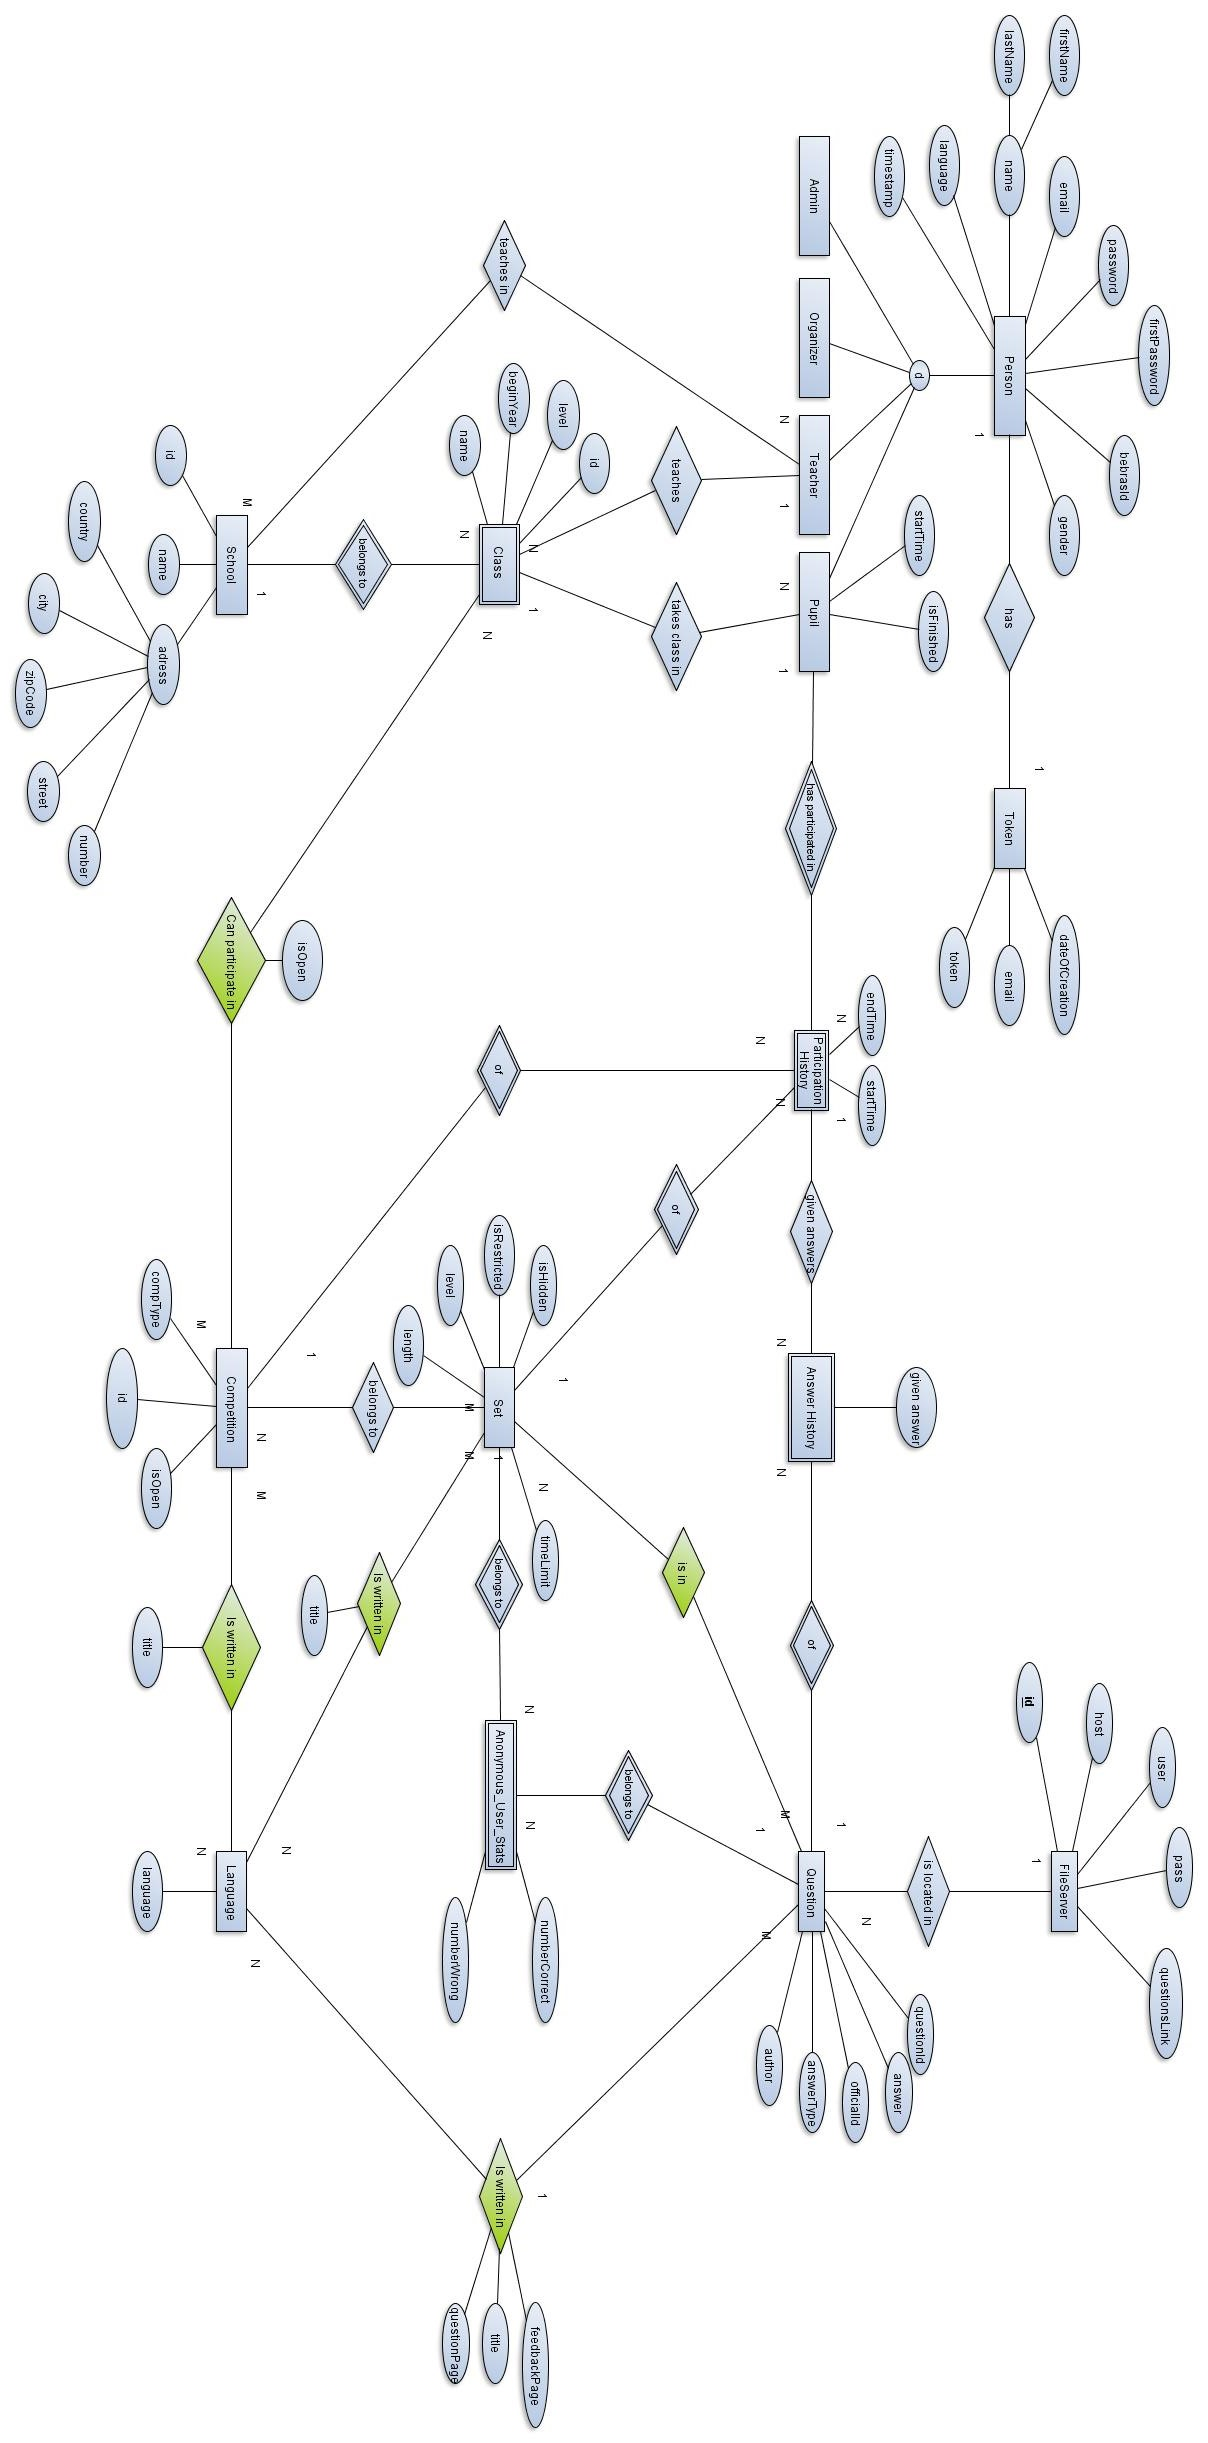
\includegraphics[scale=0.4]{eer.jpg}
\end{figure}
\end{document}